\subsection{U-Net for video segmentation}
In an attempt to make the predicted video segmentations from the 2D ResNet model more structured, a 1D U-Net was trained on the predictions of model \textit{Idx\_2\_3\_4\_5\_6\_skip\_20}. Training was conducted in a 'leave-one-out' fashion on the 25 predicted segmentations suitable for treatment predictions. The model was trained for 100 epochs with a learning rate of $3\cdot 10^{-6}$, binary cross entropy as loss function, Adam for optimization and $0.25$ weight decay.\\
The true segmentations was used as target, and was 'artificially' constructed by concatenating a vector of zeros equal in length to the number of frames up to the true separation point, and a vector of ones equal in length to the remaining frames of the video, such that we get one continuous block of inflammation predictions followed by one continuous block of healthy predictions which correspond to how the doctor annotated the video.\\
In the following, four predictions will be reported to show the effect of the trained U-Net model. In each illustration the true segmentation will be shown as the top bar, the 2D ResNet prediction will be shown as the second bar, and the 1D U-Net prediction and its confidence in a healthy prediction will be shown as the third bar.

\begin{figure}[H]
	\centering
	\begin{subfigure}{\linewidth}
		\centering
		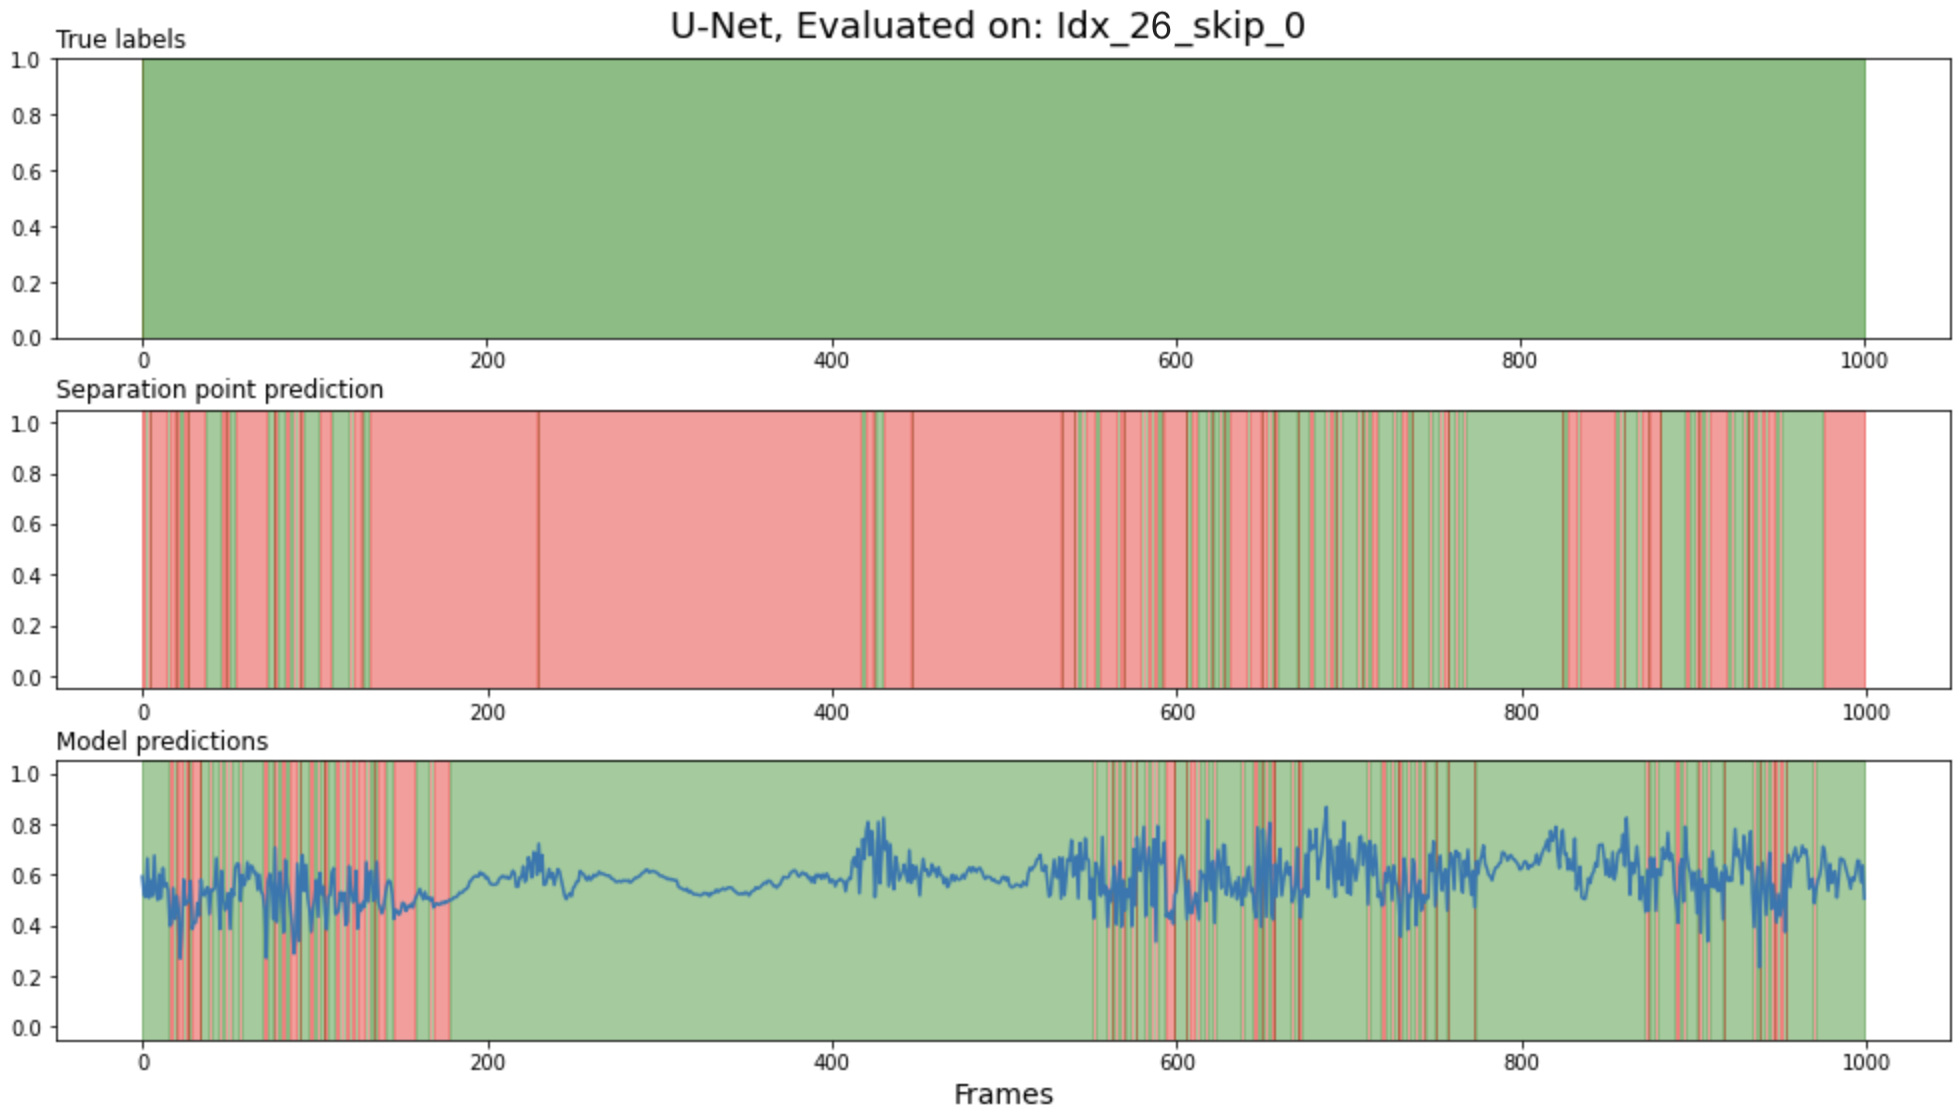
\includegraphics[width=\linewidth]{Materials/Results/UNet/unet1}
	\end{subfigure}
	\\
	\begin{subfigure}{\linewidth}
		\centering
		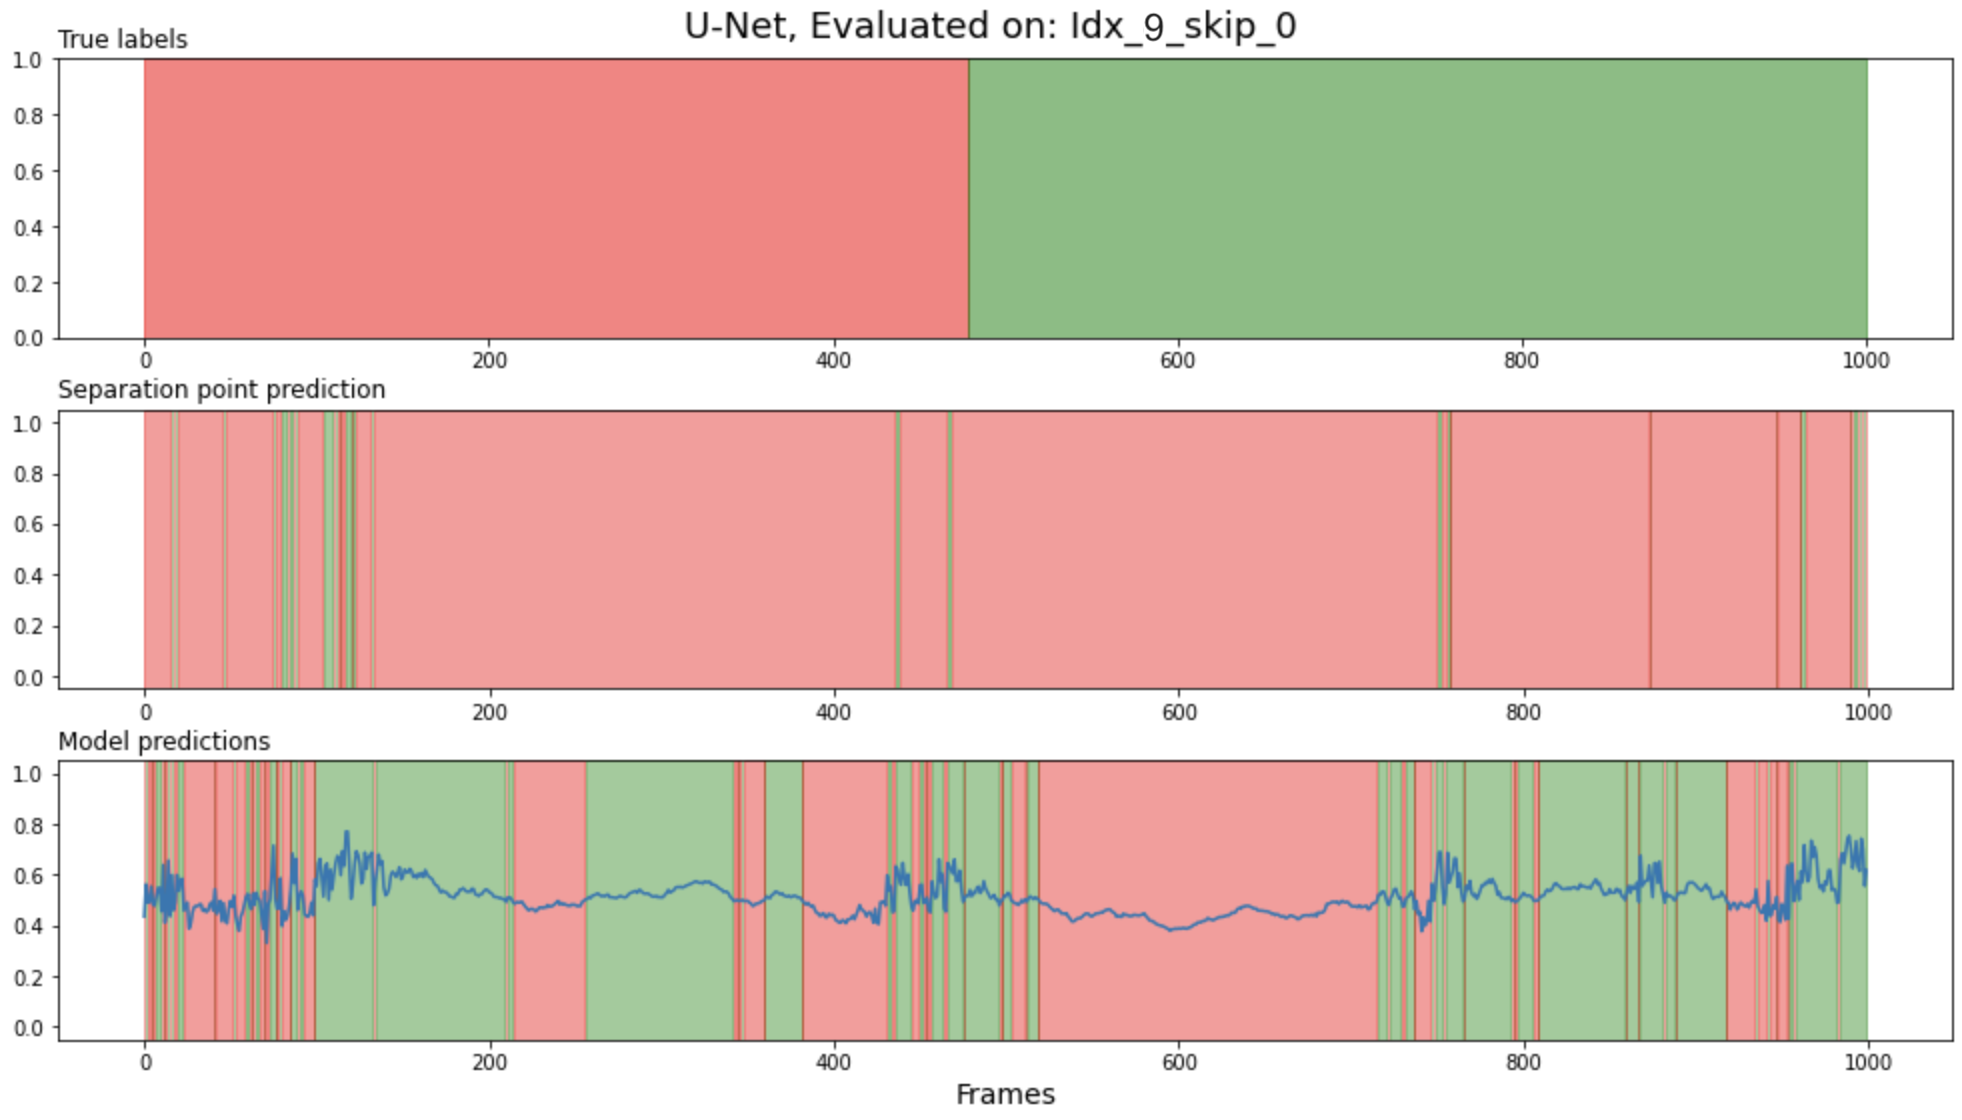
\includegraphics[width=\linewidth]{Materials/Results/UNet/unet2}
	\end{subfigure}
	\caption{Results of 1D U-Net model.}
	\label{unetres1}
\end{figure}

Taking a look at the first result presented in \autoref{unetres1}, we see the true segmentation is all healthy, but the ResNet prediction has a lot of inflammation predictions. Although the U-Net model is not confident in its predictions, it is certain in the sense it does not have very big oscillations. We also see the U-Net predictions have overturned a lot of the inflammation predictions, and made the prediction a lot more representative to the true segmentation.\\
Looking at the second prediction in \autoref{unetres1}, we see the true segmentation being almost half inflammation and half healthy. The ResNet predictions are however almost exclusively inflammation. Again we see the U-Net predictions being very steady and overturning a lot of the inflammation predictions, however this time also making correctly predicted inflamed frames healthy.

\begin{figure}[H]
	\centering
	\begin{subfigure}{\linewidth}
		\centering
		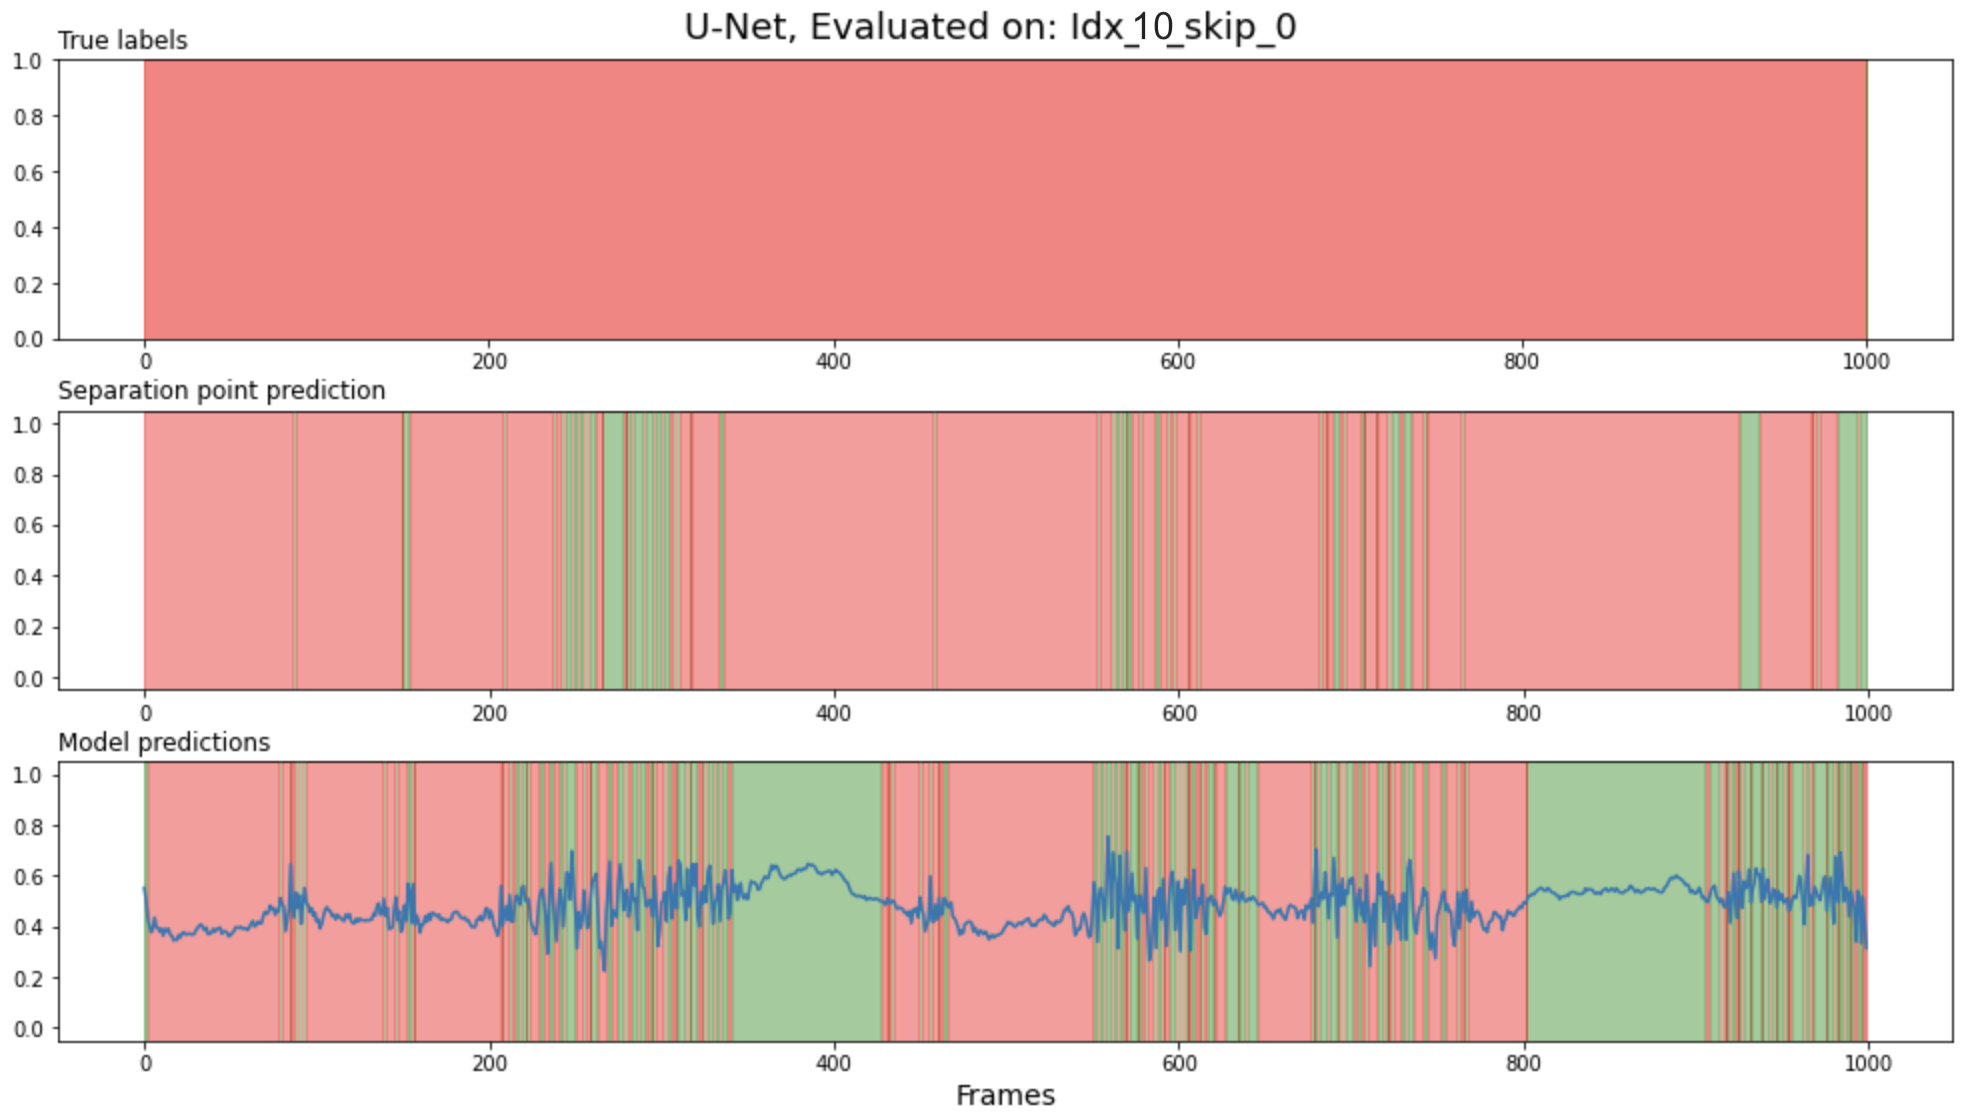
\includegraphics[width=\linewidth]{Materials/Results/UNet/unet3}
	\end{subfigure}
	\\
	\begin{subfigure}{\linewidth}
		\centering
		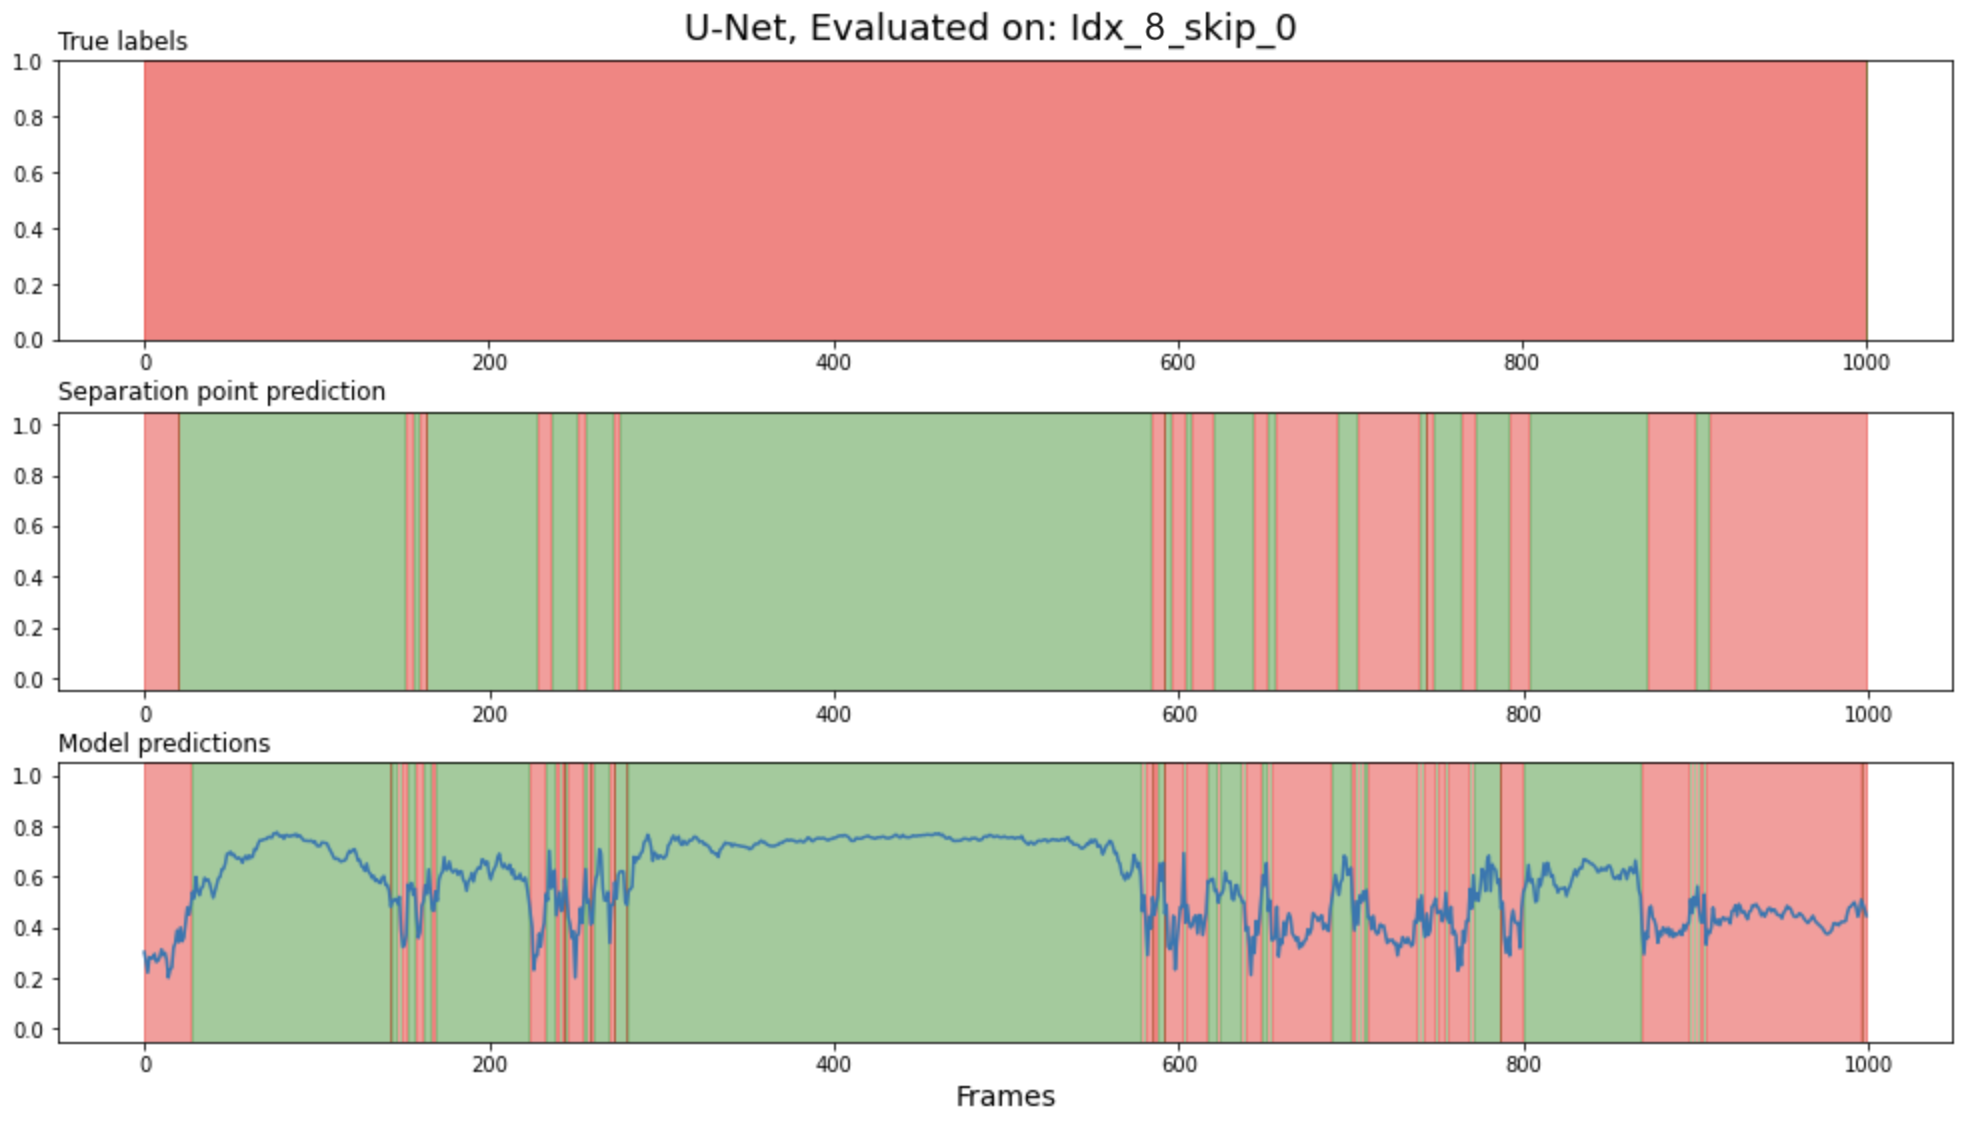
\includegraphics[width=\linewidth]{Materials/Results/UNet/unet4}
	\end{subfigure}
	\caption{Results of 1D U-Net model.}
	\label{unetres2}
\end{figure}

This tendency of making inflamed frames healthy seem to continue as we see in \autoref{unetres2}. For the first prediction we see the U-Net model likes to add healthy predictions even if they are wrong. In the second prediction we see the U-Net model is quite reluctant to add inflammation predictions when the ResNet model predicts too many healthy frames.

Even though we have only looked at four predictions this is the general tendency of the U-Net predictions. The model adds healthy predictions to the ResNet predictions, and it is very reluctant to add inflammation predictions, while being very steady and not overly confident in its predictions. As the ResNet was overly predicting inflammation, the U-Net seems to have caught on to a correct tendency of missing healthy frames. Although it has not quite managed to make its predictions two continuous blocks, its predictions are not heavily oscillating, and thus seem to have have caught on to the continuity a little.